\documentclass[11pt]{article}

\usepackage{lscape}

\usepackage{graphicx}
\begin{document}
\begin{landscape}

\begin{minipage}{0.45\textwidth}
WS: $R = \frac{U}{I} = \frac{\rho * l}{A}$; $[R] = 1\frac{V}{A} =1 \Omega$ \\
Leitwert: $G = \frac{1}{R}$\\
Maschensatz: $\sum U_i = 0$\\
Knotensatz: $\sum I_i = 0$\\
Reihe WS: $R_{ges} = \sum R_i$\\
Parallel WS: $\frac{1}{R_ges} = \sum \frac{1}{R_i}$\\
\phantom{ss} Spezialfall: $R_{ges} = \frac{R_1 * R_2}{R1+R2} $\\
V-Teiler: $\frac{U_1}{U_2} = \frac{R_1}{R_2}$\\
I-Teiler: $\frac{I_1}{I_2} = \frac{R_2}{R_1}$\\
Leistung: $P =U*I = I^2*R = \frac{U^2}{R}$ \\
\phantom{ssssssssss} $[P] = 1V*A =1 W$\\
Kondensator:\\
Kapazität: $C = \frac{Q}{U}, [C]=1F$\\
$\tau = R*C$\\
Vollständig Auf-/Entlanden: $t = 3\tau$\\
Leitungen:\\
$k_0 = \frac{R_w}{R_w + R_i} $\\
$r_a = \frac{R_a - R_w}{R_a + R_w} $\\
$k_a = 1 + r_a$\\
Anfang: $U_k(0,t)=k_0*U_{q1}(t)$\\
Ende: $U_k(x,t)= k_0*U_{q1}(t-\Delta t)$
Auskoppeln Gatter:\\
\phantom{ss} $U_1(t) = k_a * U_1(x,t)$\\
$\Delta t = l/c$\\
%Aufladen über WS: $
Koaxialkabel:\\
$R_W = \sqrt{\frac{L'}{C'}}$\\
    \phantom{ss} $=\frac{\sqrt{\epsilon_R * \mu_R}}{c_0 * C'}$\\
    \phantom{ss} $=\frac{\sqrt{\mu_R} * ln(\frac{d_a}{d_i})}{2c_0 * \pi * \epsilon_0 *\sqrt{\epsilon_R}}$
\end{minipage}%
~~~~~~~
\begin{minipage}{0.3\textwidth}

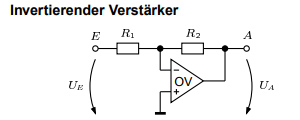
\includegraphics[scale=0.40]{IOV.png}
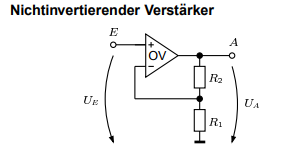
\includegraphics[scale=0.40]{NIOV.png}
$U_D = 0$
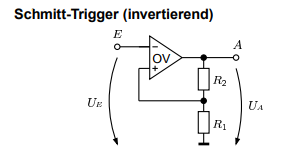
\includegraphics[scale=0.40]{ISTOV.png}
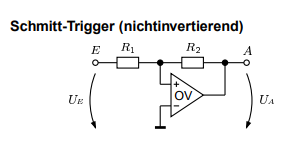
\includegraphics[scale=0.40]{NISTOV.png}
% TODO U_D = ?

\end{minipage}%
~~~~~~
\begin{minipage}{0.3\textwidth}
3. Spalte
\end{minipage}%

\end{landscape}
\end{document}
